\section{Task I : Predicting the Medal of the 2028 LA Olympics}
\subsection{Model Establishment}
Since we want to predict future medal list on the basis of past data, we merge the given data and do some preprocessing. 
We combine the data with the same \textbf{Year} and \textbf{NOC} together.

We use \textbf{Correlation Coefficient Matrix} and \textbf{Principal Component Analysis}, split the data
into training and testing parts, and use \textbf{Extreme Gradient Boosting methods} to train features
and target matrix.

We also use \textbf{KS test} to ensure the effectiveness of the model.After the model is established, we use it to predict the 2028 and 2032 Olympics.

What's important is that we add the factor of whether being a host city/country or not in to the training model so that the final result can take this factor into consideration. For example,
in the coming LA Olympics, the USA is likely to gain more medals due to the \textbf{"hosting effect"}.

\subsection{Result Analysis}

\begin{figure}[htbp]
    \centering
    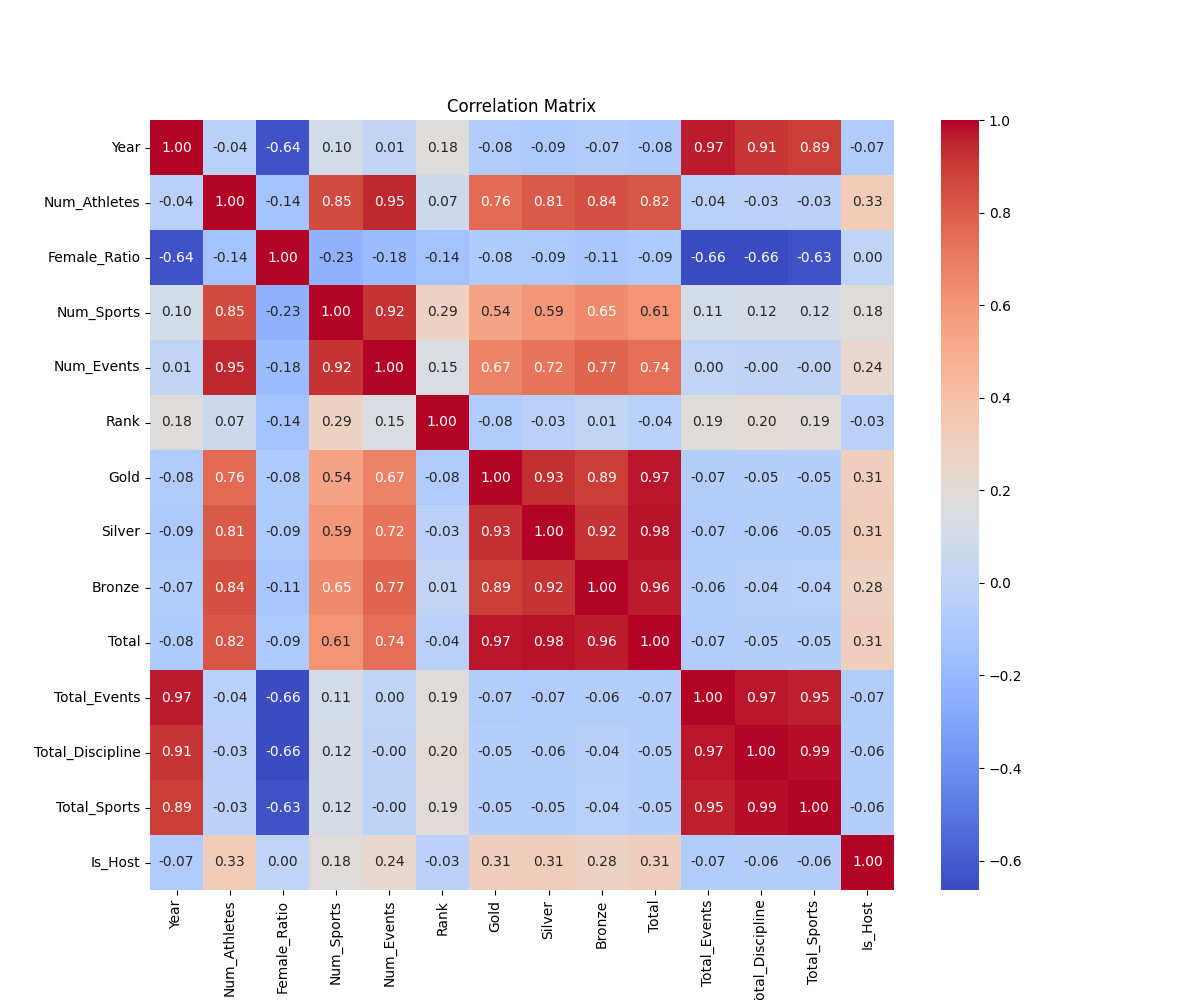
\includegraphics[width=1\textwidth]{./figures/Cor_Matrix.png}
    \caption{Correlation Matrix}
    \label{fig:Cor_Matrix}
\end{figure}

\begin{figure}[htbp]
    \centering
    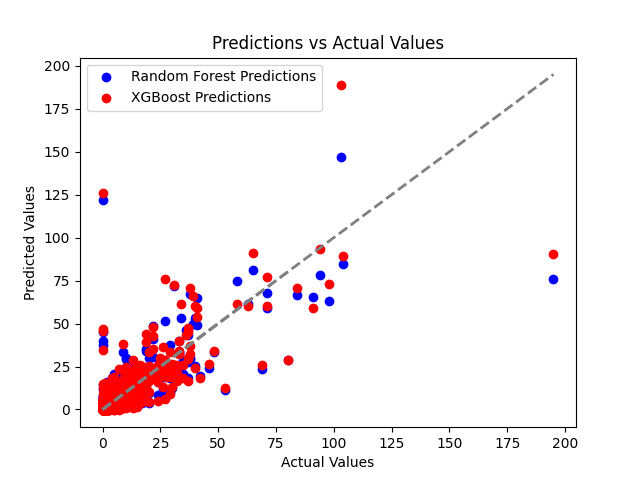
\includegraphics[width=0.8\textwidth]{./figures/K-S_0.png}
    \caption{Precision of the estimation}
    \label{fig:K-S_0}
\end{figure}

\begin{figure}[htbp]
    \centering
    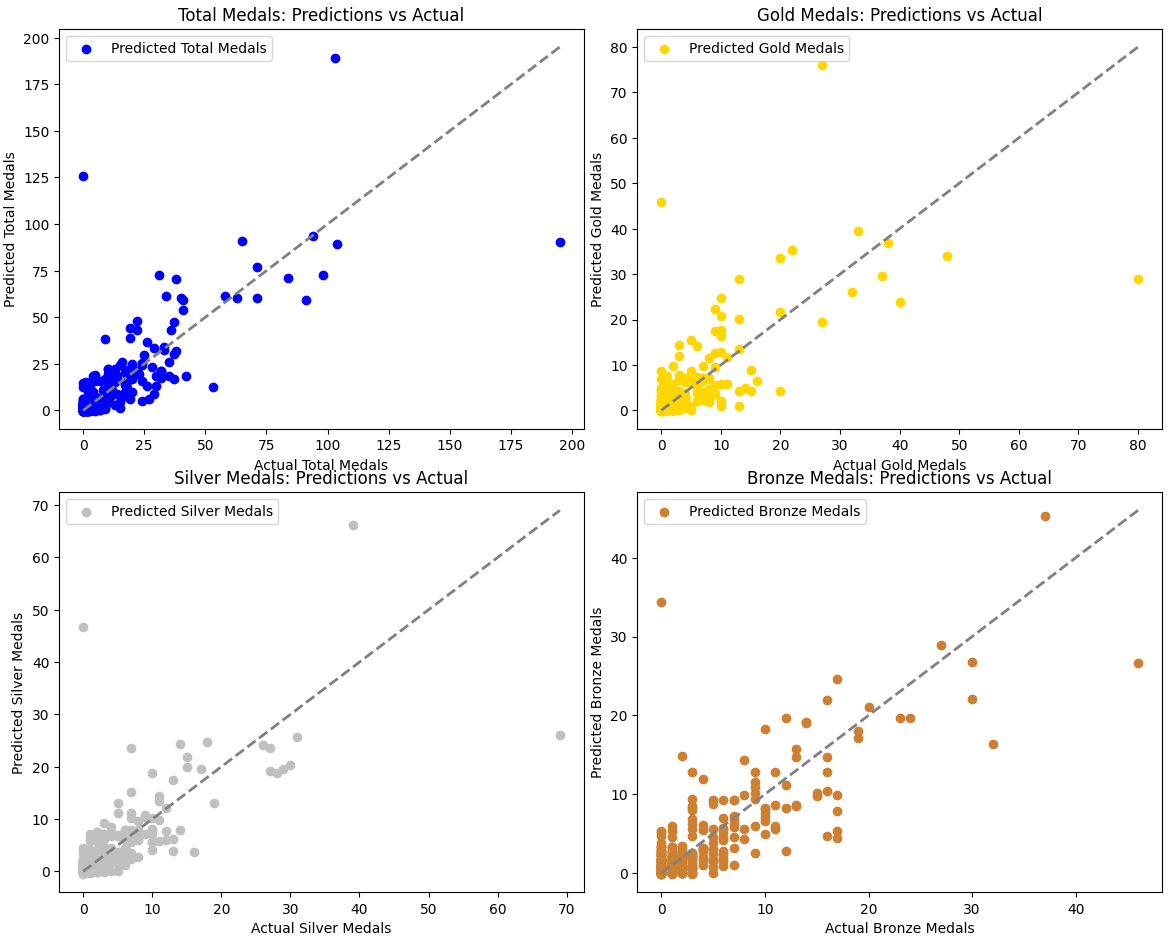
\includegraphics[width=0.8\textwidth]{./figures/K-S_4.png}
    \caption{Precision of the estimation(Gold, Silver, Bronze and Total)}
    \label{fig:K-S_4}
\end{figure}

\begin{figure}[htbp]
    \centering
    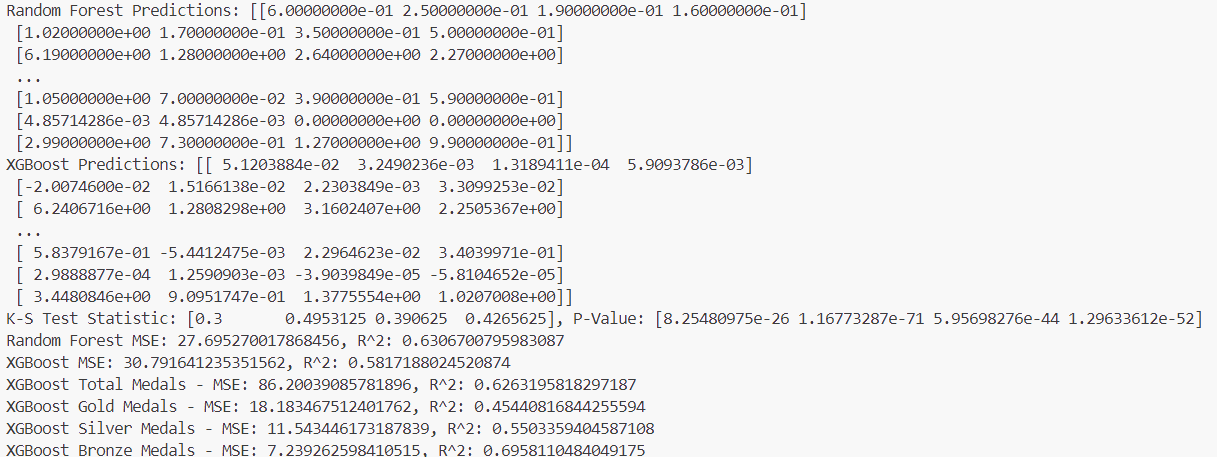
\includegraphics[width=1\textwidth]{./figures/refer_KS_other.png}
    \caption{Measures of Performance}
    \label{fig:refer_KS_other}
\end{figure}

According to the results graphs following, we can see that our model is of good accuracy, and have a good performance on test set.


From Figure2, we can see that the prediction of XGBoost outperformed the prediciton of Random Forest Predicitons, which is one of the reason for our choice of model.

As to the specific principle of XGBoost:

\begin{center}
    $\hat{y}_i^{(t)} = \hat{y}_i^{(t-1)} + f_t(x_i)$
\end{center}

The loss function and the objective function are as follows:

$L(\hat{y}_i^{(t-1)}, y_i)$ \quad \text{loss function} $y_i$ \text{prediction from the first to the t-1th tree} $\hat{y}_i^{(t-1)}$

The complete objective function (loss function plus regularization term) can be represented as:
\begin{center}
    $\mathcal{L}^{(t)} = \sum_{i=1}^n L(\hat{y}_i^{(t-1)}, y_i) + \Omega(f_t)$
\end{center}

where $\Omega(f_t)$ is the model complexity of the t-th tree, which can be expressed as:

\begin{center}
    $\Omega(f_t) = \gamma T + \frac{1}{2} \lambda \sum_{j=1}^T w_j^2$
\end{center}

where $T$ is the number of nodes in the tree, $w_j$ is the weight of each node, and $\gamma$ and $\lambda$ are regularization parameters.

\subsection{Prediction of 2028 Los Angeles Olympics}
\begin{table}[htbp]
    \centering
    \caption{Predicted Medal Table of 2028 Los Angeles Olympics}
    \begin{tabular}{|c|c|c|c|c|c|}
        \hline
        Rank & NOC & Gold & Silver & Bronze & Total \\
        \hline
        1 & United States & 49 & 46 & 44 & 139 \\
        2 & China & 38 & 30 & 29 & 97 \\
        3 & Russia & 28 & 25 & 22 & 75 \\
        4 & United Kingdom & 27 & 23 & 20 & 70 \\
        5 & Japan & 22 & 19 & 17 & 58 \\
        6 & Australia & 17 & 15 & 13 & 45 \\
        7 & Italy & 15 & 13 & 12 & 40 \\
        8 & Netherlands & 13 & 12 & 11 & 36 \\
        9 & France & 14 & 12 & 9 & 35 \\
        10 & Germany & 15 & 12 & 8 & 35 \\
        \hline
    \end{tabular}
    \label{tab:2028}
\end{table}

